\begin{figure}[t!]
\centering
\begin{tikzpicture}
\begin{axis}[
	height=2.2in,
	width= 2.6in,
	axis x line = bottom,
	axis y line = left,
	minor x tick num=10,
	ylabel={$\frac{\epsilon_i + \epsilon_{j+1}}{2}$},
	xlabel={\textbf{a}) Persistence landscape \texttt{cifar10}.},
	xmin=0,
	xmax=1050,
	ymin=0,
	ymax=650,
	ticklabel style={font=\small},
	x label style={at={(axis description cs:0.5,-0.1)},anchor=north},
	y label style={at={(axis description cs:0.20,0.85)},rotate=-90,anchor=south, fill=white},
	axis line style={-{Latex[length=1.5mm,width=1.5mm]}}
]
\coordinate (spypoint) at (axis cs:88,50);
\coordinate (magnifyglass) at (axis cs:800,400);
\draw [thick, dotted, draw=gray] (axis cs: 0,580) -- (axis cs: 1050,580) node[pos=0.9, below] {$\infty$};
\end{axis}
\begin{scope}[spy using outlines={circle, magnification=4, connect spies}]
\node[inner sep=0pt] at (2.38,1.77) {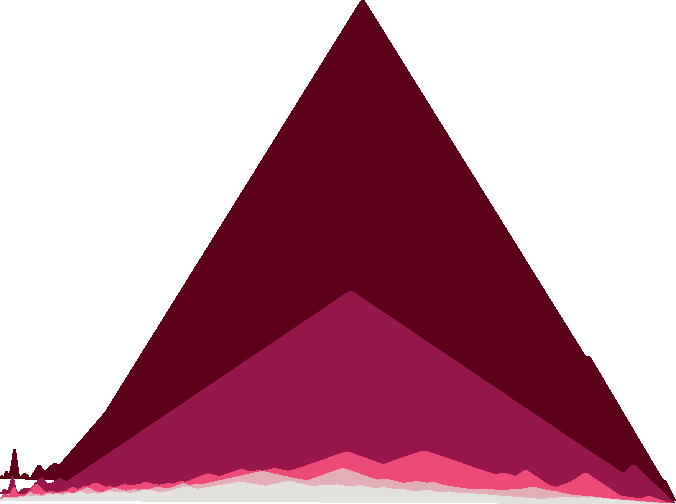
\includegraphics[width=0.39\textwidth]{figure2_a.pdf}};
\spy [lightgray, size=2cm] on (spypoint) in node[fill=white] at (magnifyglass);
\end{scope} 
\end{tikzpicture}
\begin{tikzpicture}
\begin{axis}[
	height=2.2in,
	width= 2.6in,
	axis x line = bottom,
	axis y line = left,
	minor x tick num=10,
	xlabel={\textbf{b}) Persistence landscape \texttt{cifar100}.},
	xmin=0,
	xmax=1050,
	ylabel={$\cdot 10^{3}$},
	ymin=0,
	ymax=5,
	ticklabel style={font=\small, fill=white},
	x label style={at={(axis description cs:0.5,-0.1)},anchor=north},
	y label style={at={(axis description cs:0.1,0.9)},rotate=-90,anchor=south},
	axis line style={-{Latex[length=1.5mm,width=1.5mm]}}
]
\draw [thick, dotted, draw=gray] (axis cs: 0,4.45) -- (axis cs: 1050,4.45) node[pos=0.9, below] {$\infty$};
\end{axis}
\node[inner sep=0pt] (h) at (2.38,1.77) {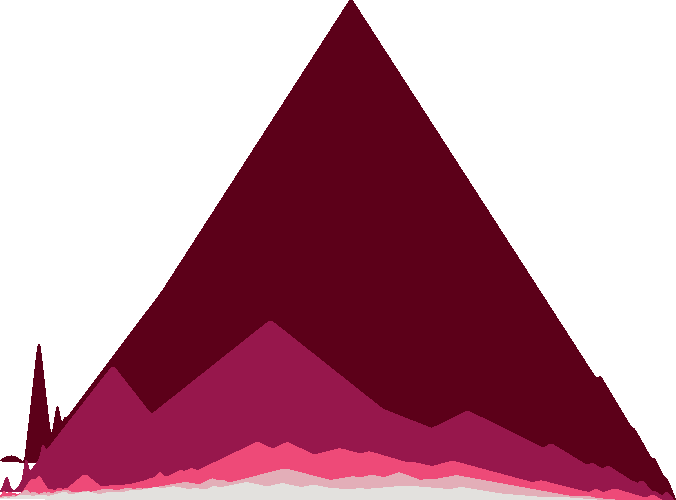
\includegraphics[width=0.39\textwidth]{figure2_b.pdf}};
\node[inner sep=0pt] (h) at (4.5,2.7) {{\color{red5}$\bullet$} {$H_0$}};
\node[inner sep=0pt] (h) at (4.5,2.3) {{\color{red4}$\bullet$} {$H_1$}};
\node[inner sep=0pt] (h) at (4.5,1.9) {{\color{red3}$\bullet$} {$H_2$}};
\node[inner sep=0pt] (h) at (4.5,1.5) {{\color{red2}$\bullet$} {$H_3$}};
\node[inner sep=0pt] (h) at (4.5,1.1) {{\color{red1}$\bullet$} {$H_4$}};
\end{tikzpicture}
\begin{tikzpicture}
	\begin{axis}[
	table/col sep=comma,
	xlabel={\textbf{c}) Validation loss \texttt{cifar10}.},
	height=2.2in,
	width= 2.6in,
   	ticklabel style={font=\small, fill=white},
	xticklabel style={rotate=90, anchor=near xticklabel},
	x label style={at={(axis description cs:0.5,-0.15)},anchor=north},
	xtick={0,0.1,0.2,0.4,0.6,0.8,1},
    xticklabels={dummy,0,50,100,150,200,250},
	]
	\end{axis}
	\node[inner sep=0pt] at (2.51,2.08) {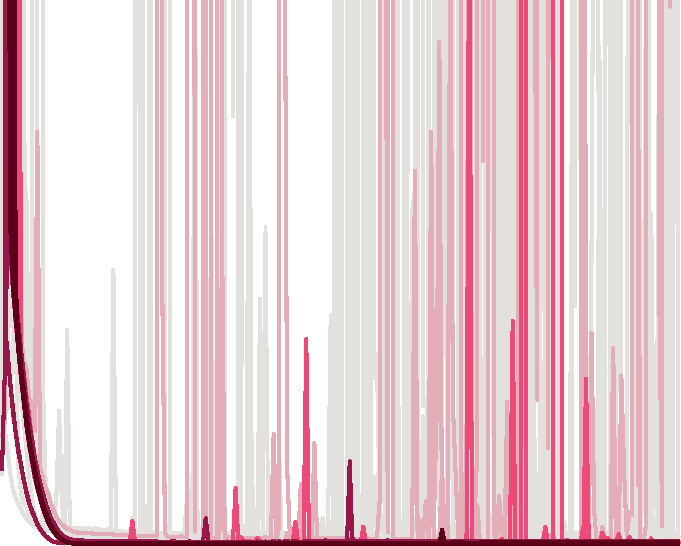
\includegraphics[width=0.343\textwidth, height=3.84cm]{figure2_c.pdf}};
\end{tikzpicture}
\begin{tikzpicture}
	\begin{axis}[
	table/col sep=comma,
	xlabel={\textbf{d}) Validation loss \texttt{cifar100}.},
	height=2.2in,
	width= 2.6in,
	ticklabel style={font=\small, fill=white},
	xticklabel style={rotate=90, anchor=near xticklabel},
	x label style={at={(axis description cs:0.5,-0.15)},anchor=north},
	xtick={0,0.1,0.2,0.4,0.6,0.8,1},
    xticklabels={dummy,0,50,100,150,200,250},
	]
	\end{axis}
	\node[inner sep=0pt] at (2.51,2.08) {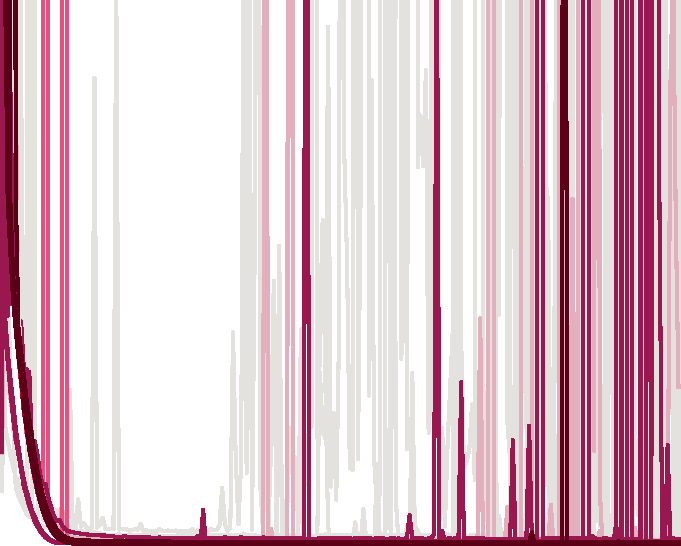
\includegraphics[width=0.343\textwidth, height=3.84cm]{figure2_d.pdf}};
\end{tikzpicture}
\caption{a) Persistence landscape for \texttt{cifar10} and b) for the \texttt{cifar100} dataset \cite{krizhevsky2009learning}. Persistence landscapes are computed up to a resolution of $10^3$. c) and d) show the \texttt{MSE} loss function on the validation dataset using a $7:3$ split on training and test data.}
\label{figure2}
\end{figure}